\begin{frame}
    \centering
    \begin{figure}[H]
        \includegraphics[keepaspectratio, width=0.7\paperwidth, height=\paperheight]{\thelogo}
    \end{figure}
    Informatik: Data Science und Sicherheit\\
    % \textbf{Lektion 4}/
    \emoji{station}: \textbf{Kürzeste Wege mit Graphen}
\end{frame}



% slide 4 (IU)
% TODO: stimmen Lernziele noch. plastische operationalisierte Lernziele
% https://www.geeksforgeeks.org/applications-of-breadth-first-traversal/
\begin{frame}[fragile]{Thema und Lernziele}
\begin{itemize}[<+->]
    \item Thema: Grundlagen der Abstraktion und Modellierung mit Graphen
    \item Lernziele:
    \begin{itemize}
        \item Sie beschreiben das Problem, möglichst kurze Wege zu finden, einem Kollegen und verwenden dabei die korrekten Fachbegriffe.
        \item Sie wenden die einzelnen Schritte des berühmten 
        
        -Algorithmus auf ein konkretes Problem an.
        %\item Sie beschreiben mindestens drei Situationen aus Ihrem Alltag, die sich mathematisch elegant modellieren lassen.
        %\item Sie erklären warum eine von Ihnen gewählte Abstraktion ein gegebenes Problem korrekt beschreibt.
    \end{itemize}
\end{itemize}
\end{frame}


% slide 5 (IU)
% TODO: tabelle mit den 4 Spalten:
% Was, Wie, Wer, Dauer
\begin{frame}[fragile]{Ablauf der Lektion}
\begin{itemize}[<+->]
    \item zuerst: Vertraut werden mit dem Thema mit Hilfe einiger Aufgaben (Sie sind gefragt!)
    \item dazwischen: Grundidee des Dijkstra-Algorithmus und Durchführung an einem Beispiel (gemeinsam)
    \item gegen Ende: Sie nutzen die Zeit für Übungen
\end{itemize}
% \begin{table}[H]
% \resizebox{1.0\textwidth}{!}{%
% \begin{tabular}{|l|l|l|l|}
% \hline
% \textbf{Was?}                                 & \textbf{Wer?} & \textbf{Wie} & \textbf{Zeit}    \\ \hline
% Einstieg                                      & gemeinsam     & Beamer       & 10 bis 15 Min.   \\ \hline
% 1. Aufgabenblock    & Sie           & Papier       & 5 Min.           \\ \hline
% kurze Besprechung der Aufgaben                & Sie           & Beamer       & 5 Min.           \\ \hline
% 2. Aufgabenblock & gemeinsam     & Papier       & 10 Min.          \\ \hline
% Beobachtung zum Brückenproblem                & gemeinsam     & Beamer       & 5 Min.           \\ \hline
% 3. Aufgabenblock                   & Sie           & Papier       & Rest der Lektion \\ \hline
% \end{tabular}%
% }%
% \end{table}
\end{frame}


% slide 6 (IU)
% TODO: meine positiven Erwartungen
% deutlich machen, wie ich das Thema finde
% Verbinden Sie das Thema mit solchen in den vergangenen oder künftigen Stunden
% Anerkennen Sie die Vorkenntnisse!
\begin{frame}[fragile]{Bemerkungen zu dem Thema} % <-- vielleicht kein Slide nötig!
\begin{itemize}[<+->]
    \item Für dieses Thema werden wir die neuen Begriffe aus der ersten Lektion verwenden.
    \item Auch der Inhalt dieses Themas ist verknüpft mit der Thematik von Webseiten und dem Internet.
    \item Sie haben in dieser Lektion die Chance die Grundzüge eines Algorithmus kennenzulernen, der sogar einen Namen hat (und somit super wichtig sein muss).
\end{itemize}
\end{frame}


\begin{frame}[fragile]{Lektion 2}
\begin{itemize}[<+->]
    \item Muss mit \enquote{kürzestem Weg} immer die Distanz gemeint sein?
    \item Sie haben die Auswahl zwischen drei verschiedenen Zugverbindungen. Für welche entscheiden Sie sich vermutlich?
\end{itemize}
\end{frame}


\begin{frame}[fragile]{Schreibweise}
\begin{figure}[H]
\centering
\begin{tikzpicture}[
node distance = 12mm and 14mm,
every state/.append style = {inner sep=0pt, fill=gray!10,
                             minimum size=11mm},
every edge/.style = {draw, -Triangle, bend angle=15},
                auto=right,
                        ]
\node (s) [state,fill=Blue!20,align=center]         {$s$};
\node (v1) [state, above right=of s,align=center]   {};
\node (v2) [state, below right=of v1,align=center]         {};
\node (t) [state,fill=Green!20, above right=of v2,xshift=-9mm,yshift=12mm,align=center]   {$t$};
% 
% \draw[gray!30, line width=5pt]
%         (s1) to                     (s2)
%         (s1) to [bend right=15]     (s6);
% 
\draw   (s) edge ["2"]             (v1)
        (v1) edge ["5"]            (v2)
        (v2) edge ["3"]              (t);
\end{tikzpicture}
    \caption*{Der Weg von $s$ nach $t$ hat die Länge (Kosten / Gewicht) 10.}
    \label{fig:xy}
\end{figure}
\noindent
\begin{itemize}
    \item Die Länge eines Weges $p$ wird mit $c(p)$ bezeichnet.
    \item Wir schreiben
\begin{align*}
    u \stackrel{p}{\rightsquigarrow} v
\end{align*}
und meinen damit einen Weg $p$ von $u$ nach $v$.
\end{itemize}
\end{frame}


\begin{frame}[fragile]{1. Aufgabenblock (10 Minuten)}
\begin{center}
    Bearbeiten Sie die vier Aufgaben 1.1, 1.2, 1.3 und 1.4.
\end{center}
\end{frame}

% Wir nehmen an, dass ein Graph nur positive Kantengewichte besitzt. Kann in diesem Graphen ein kürzester Weg von Knoten $s$ nach Knoten $t$ eine Schleife (einen \textit{Zyklus}) enthalten?
% \end{frame}


% \begin{frame}[fragile]{Beobachtung 1}
% \begin{figure}[H]
% \centering
% \begin{tikzpicture}[
% node distance = 10mm and 12mm,
% every state/.append style = {inner sep=0pt, fill=gray!10,
%                              minimum size=8mm},
% every edge/.style = {draw, -Triangle, bend angle=15},
%                 auto=right,
%                         ]
% \node (s) [state,fill=Blue!20,align=center]         {$s$};
% \node (u) [state, right=of s,align=center]   {$u$};
% \node (v) [state, above right=of u,align=center]         {$v$};
% \node (t) [state,fill=Green!20,below right=of v,align=center]   {$t$};
% \node (w) [state, below right=of u,align=center]   {$w$};
% % %
% % \draw[gray!30, line width=5pt]
% %         (s1) to                     (s2)
% %         (s1) to [bend right=15]     (s6);
% % %
% \draw   (s) edge ["1",color=Blue] (u)
%         (u) edge ["1",color=Blue] (v)
%         (v) edge ["1",color=Blue] (t)
%         (v) edge ["1"] (w)
%         (w) edge ["2"] (u)
%         (w) edge ["4"] (t);
% \end{tikzpicture}
% \end{figure}
%     \begin{align*}
%         &\textcolor{Blue}{s \longrightarrow u \longrightarrow v \longrightarrow t} \\
%         &\textcolor{Blue}{s \longrightarrow u \longrightarrow} \textcolor{Red}{ v \longrightarrow w \longrightarrow u \longrightarrow v} \textcolor{Blue}{\longrightarrow  t}\\
%     \end{align*}
% Ein Zyklus (hier: $\textcolor{Red}{ v \longrightarrow w \longrightarrow u \longrightarrow v}$) macht den Weg unnötig lange! Wir können den Zyklus einfach weglassen. Kürzeste Wege enthalten keine Zyklen.
% \end{frame}


\begin{frame}[fragile]{Beobachtung}
\begin{figure}[H]
\centering
\begin{tikzpicture}[
node distance = 22mm and 24mm,
every state/.append style = {inner sep=0pt, fill=gray!10,
                             minimum size=11mm},
every edge/.style = {draw, -Triangle, bend angle=15},
                auto=right,
                        ]
\node (s) [state,fill=Blue!20,align=center]         {$s$\\$0$};
\node (t) [state, above right=of s,align=center]   {$t$\\$8$};
\node (y) [state, below right=of s,align=center]         {$y$\\$5$};
\node (x) [state, right=of t,align=center]   {$x$\\$9$};
\node (z) [state, right=of y,align=center]   {$z$\\$7$};
%
\draw[Green!20, line width=5pt]
        (s) to                     (y)
        (y) to [bend right=15]     (t)
        (t) to                     (x)        ;
%
\draw   (s) edge ["10"]             (t)
        (s) edge ["5"]              (y)
        (t) edge ["1"]              (x)
        (t) edge [bend right,"2"]    (y)
        (y) edge [bend right,"3"]   (t)
        (y) edge ["9"]  (x)
        (y) edge ["2"]             (z)
        (x) edge [bend right,"4"]  (z)
        (z) edge [very near end,"7"]  (s)
        (z) edge [bend right,"6"]    (x);
\end{tikzpicture}
\end{figure}  
\end{frame}


\begin{frame}[fragile]{Beobachtung}
Sei $p$ der Weg $u \stackrel{p_1}{\rightsquigarrow} x \stackrel{p_2}{\rightsquigarrow} y \stackrel{p_3}{\rightsquigarrow} v$ zusammengesetzt aus den Wegen $p_1, p_2, p_3$. Angenommen $p$ sei ein kürzester Weg von $u$ nach $v$. Seien $x$ und $y$ beliebige Knoten entlang dieses Weges. Dann ist der Abschnitt $p_2$ von $x$ nach $y$ ein kürzester Weg von $x$ nach $y$.
\begin{figure}[H]
\centering
\begin{tikzpicture}[
node distance = 12mm and 14mm,
every state/.append style = {inner sep=0pt, fill=gray!10,
                             minimum size=11mm},
every edge/.style = {draw, -Triangle, bend angle=15},
                auto=right,
                        ]
\node (u) [state,align=center,]         {$u$};
\node (x) [state, right=of u,align=center]   {$x$};
\node (y) [state, right=of x,align=center]   {$y$};
\node (v) [state, right=of y,align=center]   {$v$};

% %
% \draw[gray!30, line width=5pt]
%         (s1) to                     (s2)
%         (s1) to [bend right=15]     (s6);
% %
\draw   (u) edge [decorate, decoration={snake,amplitude=.6mm,segment length=3mm,post length=2mm},"$p_1$"] (x)
(x) edge [decorate, decoration={snake,amplitude=.6mm,segment length=3mm,post length=2mm},"$p_2$"] (y)
(x) edge [bend left=50, decorate, decoration={snake,amplitude=.6mm,segment length=3mm,post length=2mm},"$q$"] (y)
(y) edge [decorate, decoration={snake,amplitude=.6mm,segment length=3mm,post length=2mm},"$p_3$"] (v);
\end{tikzpicture}
\end{figure}
% \noindent
% Wäre nämlich $q$ ein kürzerer Weg von $x$ nach $y$, dann hätten wir ja von Anfang auf dem Weg von $u$ nach $v$ diesen kürzeren Teilweg nehmen können!
\end{frame}


% \begin{frame}[fragile]{negative Kantengewichte}
% \begin{figure}[H]
% \centering
% \begin{tikzpicture}[
% node distance = 20mm and 24mm,
% every state/.append style = {inner sep=0pt, fill=gray!10,
%                              minimum size=11mm},
% every edge/.style = {draw, -Triangle, bend angle=15},
%                 auto=right,
%                         ]
% \node (s) [state,fill=Blue!20,align=center]         {$s$};
% \node (v1) [state, above right=of s,align=center]   {};
% \node (v2) [state, below right=of v1,align=center]         {};
% \node (t) [state,fill=Green!20, above right=of v2,xshift=-9mm,yshift=12mm,align=center]   {$t$};
% % 
% % \draw[gray!30, line width=5pt]
% %         (s1) to                     (s2)
% %         (s1) to [bend right=15]     (s6);
% % 
% \draw   (s) edge ["5"]             (v1)
%         (v1) edge ["-2"]            (v2)
%         (v2) edge ["3"]              (t);
% \end{tikzpicture}
% \end{figure}
% \end{frame}



\begin{frame}[fragile]{Dijkstra-Algorithmus}
\begin{figure}
    \centering
    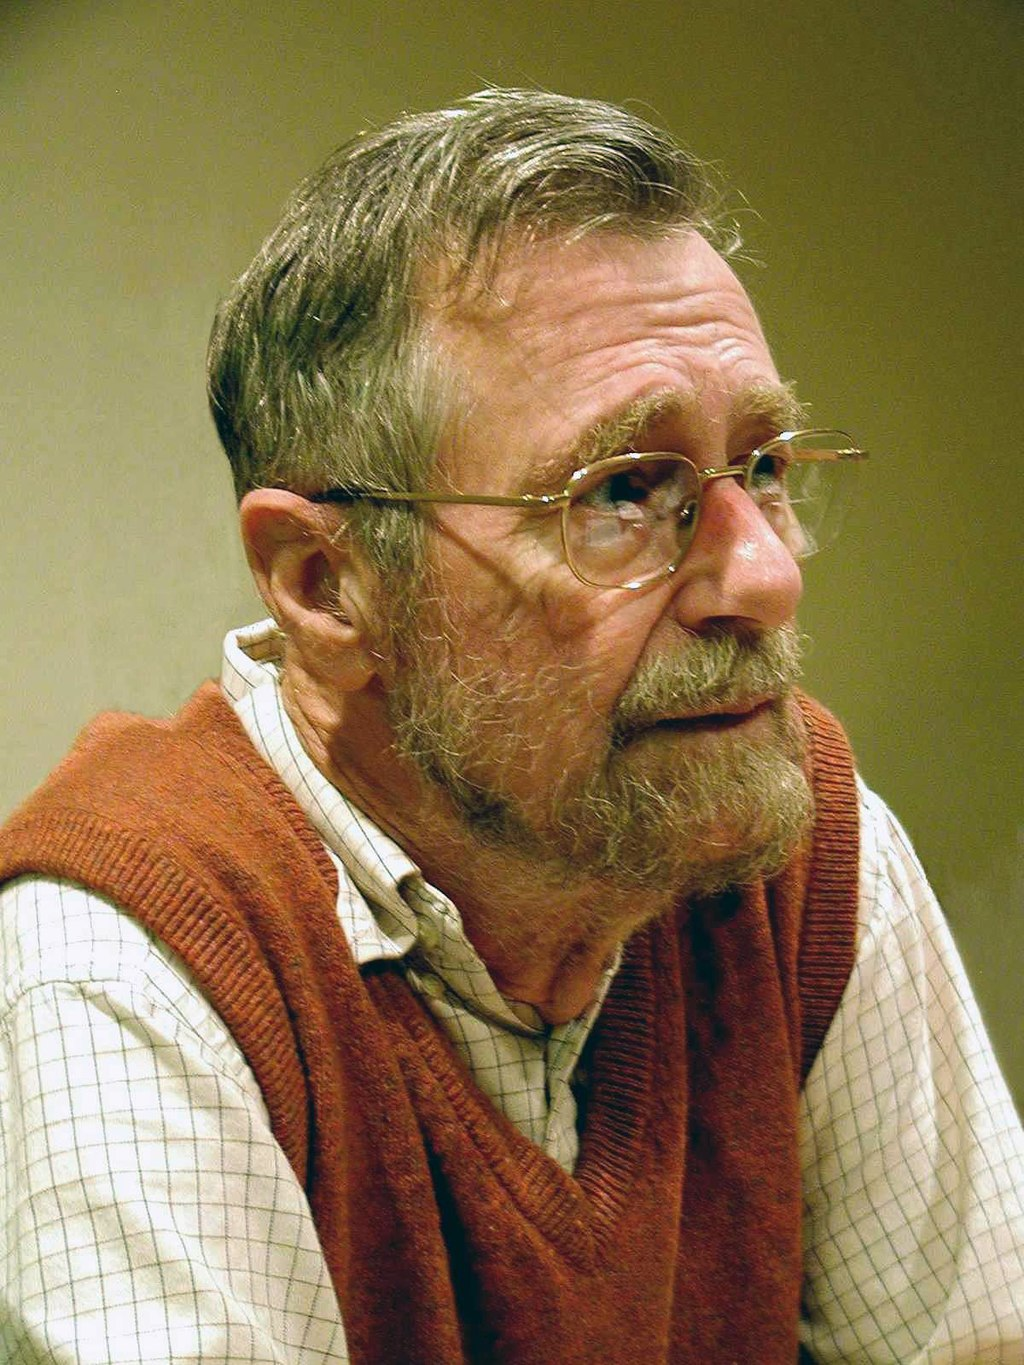
\includegraphics[width=0.5\textwidth]{Grundlagen_Info/02_Graphen/AbstraktionDurchGraphen/Figures/Edsger_Wybe_Dijkstra.jpg}
    \caption*{Edsger Wybe Dijkstra}
\end{figure}
\end{frame}


\begin{frame}[fragile]{Dijkstra-Algorithmus}
\begin{itemize}[<+->]
    \item Wir wollen die Längen (Kosten) der jeweils kürzesten Wege von $s$ (Startknoten) zu allen anderen Knoten in einem Graphen finden. Wir werden nur noch Graphen mit nicht-negativen Kantengewichten anschauen.
    \item Computer sind enorm schnell. Warum berechnen sie nicht einfach die Länge jedes Weges und wählen einen kürzesten aus?
\end{itemize}
\end{frame}

\newcommand{\convexpath}[2]{
[   
    create hullnodes/.code={
        \global\edef\namelist{#1}
        \foreach [count=\counter] \nodename in \namelist {
            \global\edef\numberofnodes{\counter}
            \node at (\nodename) [draw=none,name=hullnode\counter] {};
        }
        \node at (hullnode\numberofnodes) [name=hullnode0,draw=none] {};
        \pgfmathtruncatemacro\lastnumber{\numberofnodes+1}
        \node at (hullnode1) [name=hullnode\lastnumber,draw=none] {};
    },
    create hullnodes
]
($(hullnode1)!#2!-90:(hullnode0)$)
\foreach [
    evaluate=\currentnode as \previousnode using \currentnode-1,
    evaluate=\currentnode as \nextnode using \currentnode+1
    ] \currentnode in {1,...,\numberofnodes} {
-- ($(hullnode\currentnode)!#2!-90:(hullnode\previousnode)$)
  let \p1 = ($(hullnode\currentnode)!#2!-90:(hullnode\previousnode) - (hullnode\currentnode)$),
    \n1 = {atan2(\y1,\x1)},
    \p2 = ($(hullnode\currentnode)!#2!90:(hullnode\nextnode) - (hullnode\currentnode)$),
    \n2 = {atan2(\y2,\x2)},
    \n{delta} = {-Mod(\n1-\n2,360)}
  in 
    {arc [start angle=\n1, delta angle=\n{delta}, radius=#2]}
}
-- cycle
}

\begin{frame}[fragile]{Grundidee}
\begin{figure}[H]
\centering
\begin{tikzpicture}[scale=1.5]
\tikzstyle{n} = [circle, draw,minimum size=.7cm]
\node[n, Maroon] (s) at (0,1) {s};
\node[n, Maroon] (l11) at (1,2) {};
\node[n, Maroon] (l12) at (1,1) {};
\node[n, Blue] (l13) at (1,0) {};
\node[n, Blue] (l21) at (2,2) {};
\node[n, Blue] (l22) at (2,1) {};
\node[n, Dandelion] (l31) at (2.5,0) {};
\node[n, Dandelion] (l32) at (3,1) {};
	  
\draw[->] (s) --node [midway,above]{2} (l11);
\draw[->] (s) --node [midway,above]{2} (l12);
\draw[->] (s) --node [midway,above]{5} (l13);
\draw[->] (l11) --node [midway,above]{3} (l21);
\draw[->] (l12) --node [midway,above]{5} (l22);
\draw[->] (l22) --node [midway,above]{2} (l32);
\draw[->] (l13) --node [midway,above]{1} (l31);
\draw[->] (l31) --node [midway,above]{2} (l32);

% Draw the colored shadow using pgfonlayer and custom convexpath function
\begin{pgfonlayer}{background}
\fill[fill=yellow!20] \convexpath{s,l11,l21,l32,l31,l13}{.3cm};
\fill[fill=blue!20] \convexpath{s,l11,l21, l22, l13}{.3cm};
\fill[fill=red!20] \convexpath{s,l11,l12}{.3cm};
\end{pgfonlayer}

\end{tikzpicture}
\end{figure}
\begin{itemize}[<+->]
    \item Die Distanzen der roten Knoten sind bereits optimal und werden sich nicht mehr ändern (nicht offensichtlich).
    \item Ebenfalls sehr wichtig: Updates der Distanzen!
\end{itemize}
\end{frame}

\begin{frame}[fragile]{Djkstra: \textit{step by step}}
	\begin{figure}[H]
		\centering
		\begin{tikzpicture}[
		node distance = 22mm and 24mm,
		every state/.append style = {inner sep=0pt, fill=gray!10,
		                             minimum size=11mm},
		every edge/.style = {draw, -Triangle, bend angle=15},
		                auto=right,
		                        ]
		\node (s) [state, fill=Yellow!50, align=center]         {$s$\\$0$};
		\node (t) [state, fill=Yellow!20, above right=of s,align=center]   {$t$\\$\infty$};
		\node (y) [state, fill=Yellow!20, below right=of s,align=center]         {$y$\\$\infty$};
		\node (x) [state, fill=Yellow!20, right=of t,align=center]   {$x$\\$\infty$};
		\node (z) [state, fill=Yellow!20, right=of y,align=center]   {$z$\\$\infty$};
		
		\draw[Green!20, line width=5pt]
		        (s) to                     (t)
		        (s) to					   (y);
		        
		\draw   (s) edge ["10"]             (t)
		        (s) edge ["5"]              (y)
		        (t) edge ["1"]              (x)
		        (t) edge [bend right,"2"]    (y)
		        (y) edge [bend right,"3"]   (t)
		        (y) edge ["9"]  (x)
		        (y) edge ["2"]             (z)
		        (x) edge [bend right,"4"]  (z)
		        (z) edge [very near end,"7"]  (s)
		        (z) edge [bend right,"6"]    (x);
		\end{tikzpicture}
		\caption*{Schritt 1}
	\end{figure}  
\end{frame}

\begin{frame}[fragile]{Djkstra: \textit{step by step}}
	\begin{figure}[H]
		\centering
			\begin{tikzpicture}[
			node distance = 22mm and 24mm,
			every state/.append style = {inner sep=0pt, fill=gray!10,
			                             minimum size=11mm},
			every edge/.style = {draw, -Triangle, bend angle=15},
			                auto=right,
			                        ]
			\node (s) [state,fill=Red!20, align=center]         {$s$\\$0$};
			\node (t) [state,fill=Blue!20, above right=of s,align=center]   {$t$\\$10$};
			\node (y) [state,fill=Blue!20, below right=of s,align=center]         {$y$\\$5$};
			\node (x) [state,fill=Yellow!20, right=of t,align=center]   {$x$\\$\infty$};
			\node (z) [state,fill=Yellow!20, right=of y,align=center]   {$z$\\$\infty$};
			
			\draw[Green!20, line width=5pt]
			        (s) to                     (t)
			        (s) to					   (y);
			
			\draw   (s) edge ["10"]             (t)
			        (s) edge ["5"]              (y)
			        (t) edge ["1"]              (x)
			        (t) edge [bend right,"2"]    (y)
			        (y) edge [bend right,"3"]   (t)
			        (y) edge ["9"]  (x)
			        (y) edge ["2"]             (z)
			        (x) edge [bend right,"4"]  (z)
			        (z) edge [very near end,"7"]  (s)
			        (z) edge [bend right,"6"]    (x);
			\end{tikzpicture}
		\caption*{Schritt 2}
	\end{figure}  
\end{frame}

\begin{frame}[fragile]{Djkstra: \textit{step by step}}
	\begin{figure}[H]
		\centering
				\begin{tikzpicture}[
				node distance = 22mm and 24mm,
				every state/.append style = {inner sep=0pt, fill=gray!10,
				                             minimum size=11mm},
				every edge/.style = {draw, -Triangle, bend angle=15},
				                auto=right,
				                        ]
				\node (s) [state, fill=Red!20, align=center]         {$s$\\$0$};
				\node (t) [state, fill=Blue!20, above right=of s,align=center]   {$t$\\$8$};
				\node (y) [state, fill=Red!20, below right=of s,align=center]         {$y$\\$5$};
				\node (x) [state, fill=Blue!20, right=of t,align=center]   {$x$\\$14$};
				\node (z) [state, fill=Blue!20, right=of y,align=center]   {$z$\\$7$};
				
				\draw[Green!20, line width=5pt]
				        (s) to					   (y)
				        (y) to					   (x)
				        (y) to					   (z)
				        (y) to	[bend right=15]    (t);
				
				\draw   (s) edge ["10"]             (t)
				        (s) edge ["5"]              (y)
				        (t) edge ["1"]              (x)
				        (t) edge [bend right,"2"]    (y)
				        (y) edge [bend right,"3"]   (t)
				        (y) edge ["9"]  (x)
				        (y) edge ["2"]             (z)
				        (x) edge [bend right,"4"]  (z)
				        (z) edge [very near end,"7"]  (s)
				        (z) edge [bend right,"6"]    (x);
				\end{tikzpicture}
		\caption*{Schritt 3}
	\end{figure}  
\end{frame}

\begin{frame}[fragile]{Djkstra: \textit{step by step}}
	\begin{figure}[H]
		\centering
				\begin{tikzpicture}[
				node distance = 22mm and 24mm,
				every state/.append style = {inner sep=0pt, fill=gray!10,
				                             minimum size=11mm},
				every edge/.style = {draw, -Triangle, bend angle=15},
				                auto=right,
				                        ]
				\node (s) [state, fill=Red!20, align=center]         {$s$\\$0$};
				\node (t) [state, fill=Blue!20, above right=of s,align=center]   {$t$\\$8$};
				\node (y) [state, fill=Red!20, below right=of s,align=center]         {$y$\\$5$};
				\node (x) [state, fill=Blue!20, right=of t,align=center]   {$x$\\$13$};
				\node (z) [state, fill=Red!20, right=of y,align=center]   {$z$\\$7$};
				
				\draw[Green!20, line width=5pt]
				        (s) to					   (y)
				        (y) to					   (z)
				        (y) to	[bend right=15]    (t)
				        (z) to	[bend right=15]    (x);
				
				\draw   (s) edge ["10"]             (t)
				        (s) edge ["5"]              (y)
				        (t) edge ["1"]              (x)
				        (t) edge [bend right,"2"]    (y)
				        (y) edge [bend right,"3"]   (t)
				        (y) edge ["9"]  (x)
				        (y) edge ["2"]             (z)
				        (x) edge [bend right,"4"]  (z)
				        (z) edge [very near end,"7"]  (s)
				        (z) edge [bend right,"6"]    (x);
				\end{tikzpicture}
		\caption*{Schritt 4}
	\end{figure}  
\end{frame}

\begin{frame}[fragile]{Djkstra: \textit{step by step}}
	\begin{figure}[H]
		\centering
			\begin{tikzpicture}[
				node distance = 22mm and 24mm,
				every state/.append style = {inner sep=0pt, fill=gray!10,
				                             minimum size=11mm},
				every edge/.style = {draw, -Triangle, bend angle=15},
				                auto=right,
				                        ]
				\node (s) [state, fill=Red!20, align=center]         {$s$\\$0$};
				\node (t) [state, fill=Red!20, above right=of s,align=center]   {$t$\\$8$};
				\node (y) [state, fill=Red!20, below right=of s,align=center]         {$y$\\$5$};
				\node (x) [state, fill=Blue!20, right=of t,align=center]   {$x$\\$9$};
				\node (z) [state, fill=Red!20, right=of y,align=center]   {$z$\\$7$};
				
				\draw[Green!20, line width=5pt]
				        (s) to					   (y)
				        (y) to					   (z)
				        (t) to					   (x)
				        (y) to	[bend right=15]    (t);
				
				\draw   (s) edge ["10"]             (t)
				        (s) edge ["5"]              (y)
				        (t) edge ["1"]              (x)
				        (t) edge [bend right,"2"]    (y)
				        (y) edge [bend right,"3"]   (t)
				        (y) edge ["9"]  (x)
				        (y) edge ["2"]             (z)
				        (x) edge [bend right,"4"]  (z)
				        (z) edge [very near end,"7"]  (s)
				        (z) edge [bend right,"6"]    (x);
				\end{tikzpicture}
		\caption*{Schritt 5}
	\end{figure}  
\end{frame}

\begin{frame}[fragile]{Djkstra: \textit{step by step}}
	\begin{figure}[H]
		\centering
			\begin{tikzpicture}[
				node distance = 22mm and 24mm,
				every state/.append style = {inner sep=0pt, fill=gray!10,
				                             minimum size=11mm},
				every edge/.style = {draw, -Triangle, bend angle=15},
				                auto=right,
				                        ]
				\node (s) [state, fill=Red!20, align=center]         {$s$\\$0$};
				\node (t) [state, fill=Red!20, above right=of s,align=center]   {$t$\\$8$};
				\node (y) [state, fill=Red!20, below right=of s,align=center]         {$y$\\$5$};
				\node (x) [state, fill=Red!20, right=of t,align=center]   {$x$\\$9$};
				\node (z) [state, fill=Red!20, right=of y,align=center]   {$z$\\$7$};
				
				\draw[Green!20, line width=5pt]
				        (s) to					   (y)
				        (y) to					   (z)
				        (t) to					   (x)
				        (y) to	[bend right=15]    (t);
				        
				\draw   (s) edge ["10"]             (t)
				        (s) edge ["5"]              (y)
				        (t) edge ["1"]              (x)
				        (t) edge [bend right,"2"]    (y)
				        (y) edge [bend right,"3"]   (t)
				        (y) edge ["9"]  (x)
				        (y) edge ["2"]             (z)
				        (x) edge [bend right,"4"]  (z)
				        (z) edge [very near end,"7"]  (s)
				        (z) edge [bend right,"6"]    (x);
				\end{tikzpicture}
		\caption*{Schritt 6}
	\end{figure}  
\end{frame}



\begin{frame}[fragile]{Initialisierung (Startbedingungen)}
Wir bezeichnen mit $d_s\lrs{v}$ die Länge des kürzesten \textbf{bisher} gefunden Weges vom Startknoten $s$ zum Knoten $v$. Mit $c(u,v)$ bezeichnen wir das Gewicht (cost) der Kante von Knoten $u$ zum Knoten $v$.
\begin{itemize}
    \item Zu Beginn: $d_s\lrs{v} = \infty$ für alle Knoten des Graphen. (Initialisierung)
    \item Ziel: Für jeden Knoten $v$ des Graphen soll am Ende $d_s\lrs{v}$ die Länge eines kürzesten Weges von $s$ nach $v$ sein. (rote Knoten)
\end{itemize}
\end{frame}

\begin{frame}[fragile]{Dijkstra-Algorithmus (informal)}
\begin{itemize}
    \item Wir fügen $u:=s$ zur roten Menge hinzu und betrachten alle Knoten, welche direkt über eine einzige Kante von $s$ aus erreichbar sind (also genau die Knoten in der blauen Menge).
    \item Für jeden dieser blauen Knoten $v$ schauen wir, ob die Bedingung
    \begin{align*}
        d_s[u] + c(u,v) < d_s[v]
    \end{align*}
    erfüllt ist. Diese Bedingung hat die Bedeutung, dass die bislang berechneten Länge $d_s[v]$ grösser ist, als wenn wir von $s$ über $u$ nach $v$ gehen würden. Trifft diese zu, so führen wir das Update
    \begin{align*}
        d_s[v] = d_s[u] + c(u,v)
    \end{align*}
    durch und verbessern dadurch den bisherigen Wert $d_s[v]$.
\end{itemize}
\end{frame}

\begin{frame}[fragile]{}
\begin{itemize}
    \item Nun wählen wir denjenigen blauen Knoten $u$, welchen den (einen der) kleinsten Werte $d_s[u]$ unter allen blauen Knoten hat, als den neuen Knoten $u$ und fügen $u$ zur roten Menge hinzu.
    \item Wir arbeiten nun so weiter, bis keine blauen Knoten mehr übrig sind.
\end{itemize}
\end{frame}

\begin{frame}[fragile]{wichtige Eigenschaft}
Eine entscheidende Tatsache in dem Algorithmus (dies ist nicht völlig offensichtlich) ist, dass die roten Knoten $v$ ihren Wert $d_s[v]$ nie mehr ändern werden und dass für sie in der Tat  $d_s\lrs{v}$ die Länge eines kürzesten Weges von $s$ nach $v$ ist.
\end{frame}


\begin{frame}[fragile]{2. Aufgabenblock (Zeit: Rest der Lekltion)}
\begin{center}
    Bearbeiten Sie die drei Aufgaben 1.5, 1.6 und 1.7.
\end{center}
\end{frame}

\begin{frame}[fragile]{}
\begin{center}
Vielen Dank!
\end{center}
\end{frame}


\begin{frame}[fragile]{Pseudocode}
\lstset{basicstyle=\ttfamily\footnotesize}
\begin{lstlisting}[language=Python,numbers=none,escapeinside={(*}{*)}]
## Initialisierung ##
für alle Knoten u des Graphen setze:
    (*$d_s[u] = \infty$*)
(*$d_s[s] \leftarrow 0$*)
(*$S \leftarrow \emptyset$*)
(*$Q \leftarrow $*) alle Knoten des Graphen

## Schritte ##
solange (*$Q$*) nicht leer ist, mach:
    (*$u\leftarrow$*) Knoten aus (*$Q$*) mit kleinstem (*$d_s[u]$*)
    (*$S\leftarrow S \cup \lrc{u}$*)

    für alle von (*$u$*) direkt erreichbaren Knoten (*$v$*) mach:
        # ist der Weg von (*$s$*) nach (*$v$*) kürzer über (*$u$*)?
        falls (*$d_s[u] + c(u,v) < d_s[v]$*) dann:
            (*$d_s[v] \leftarrow d_s[u] + c(u,v)$*)
\end{lstlisting}
\lstset{basicstyle=\ttfamily\scriptsize}
\end{frame}